\section{Observability analysis}
\label{sec:observability}

Section~\ref{sec:identifiability} established that the depletion
calibration at a fixed operating point collapses the parameter
space to a one-dimensional manifold parameterized by the
rate-source-dependent quantity $\alpha$, and
Section~\ref{sec:boltzmann} verified that Maxwellian and two-term
Boltzmann rate sources correspond to two distinct points on this
manifold that reproduce the calibration anchors to the tolerance
of the numerical fit. The two points are numerically
indistinguishable for any etch-rate measurement taken at the
calibration $E/N$, and this is not a coincidence but a structural
consequence of the identifiability theorem. A question then arises
at the experimental level: if the calibration cannot determine
which point on the manifold corresponds to the physically realized
state, what measurement can?

We address this question by defining the observable difference
between the two calibrated models at an arbitrary operating point
$\mathbf{q} = (P, E/N, x_{\mathrm{Ar}}, p)$ as
\begin{equation}
  \Delta_{\mathrm{obs}}(\mathbf{q})
  \;\equiv\;
  \frac{r_{\mathrm{Bolt}}(\mathbf{q}) - r_{\mathrm{Max}}(\mathbf{q})}
       {r_{\mathrm{Max}}(\mathbf{q})},
  \label{eq:delta-obs}
\end{equation}
where $r_{\mathrm{Max}}$ and $r_{\mathrm{Bolt}}$ are the etch rates
predicted by the Maxwellian-calibrated and Boltzmann-calibrated
models, respectively, each evaluated at $\mathbf{q}$ as a forward
prediction. At the calibration anchors
$\Delta_{\mathrm{obs}} \equiv 0$ by construction. At any point
where the two calibrated models diverge,
$|\Delta_{\mathrm{obs}}|$ is the fractional etch-rate signal an
experimenter would need to resolve in order to distinguish the two
EEDF hypotheses.

Two independent off-anchor perturbations are of experimental
interest: variation of $E/N$ at fixed Ar fraction, and variation of
$x_{\mathrm{Ar}}$ at fixed $E/N$. Varying $E/N$ changes the mean
electron energy and therefore the competition between the
attachment losses that deplete the Boltzmann-EEDF tail and the
electron heating that replenishes it. Varying $x_{\mathrm{Ar}}$
changes the weight of attachment relative to elastic momentum
transfer: Ar is a nearly elastic scatterer below its first
excitation threshold while \sfsix{} is strongly attaching, so
increasing $x_{\mathrm{Ar}}$ softens the attachment-induced tail
depletion directly. Variation of $E/N$ probes the energy axis of
the EEDF; variation of $x_{\mathrm{Ar}}$ probes the
attaching/non-attaching mixture.

Figure~\ref{fig:observability} shows $\Delta_{\mathrm{obs}}$ for
both perturbation types with both calibrated models held at the
values reported in Section~\ref{sec:boltzmann}. Along the $E/N$
axis at pure \sfsix{} and $P = 200\,$W, the discrepancy grows
rapidly as $E/N$ is reduced below the calibration value of
$100\,$Td, reaching $\Delta_{\mathrm{obs}} = -84.84\,\%$ at
$50\,$Td. The Boltzmann-calibrated model predicts only
$4.7\,$nm\,min$^{-1}$ at that operating point, against
$31.2\,$nm\,min$^{-1}$ from the Maxwellian-calibrated model. The
physical origin is sharp: at
$T_e^{\mathrm{eff}} \approx 0.7\,$eV the two-term Boltzmann EEDF
has almost no population above the $\sim9\,$eV dissociation
threshold, so $\kdiss^{\mathrm{Bolt}}$ collapses to a value four
orders of magnitude below $\kdiss^{\mathrm{Max}}$. At higher $E/N$
the discrepancy reverses sign, reaching
$\Delta_{\mathrm{obs}} = +24.72\,\%$ at $200\,$Td and $+39.62\,\%$
at $300\,$Td. The strongest $E/N$-axis observability is therefore
at the low-$E/N$ end, with a signal-to-noise ratio exceeding any
plausible experimental uncertainty by more than an order of
magnitude.

Along the $x_{\mathrm{Ar}}$ axis at $E/N = 100\,$Td and
$P = 200\,$W, the discrepancy grows monotonically from
$\Delta_{\mathrm{obs}} = 0$ at $x_{\mathrm{Ar}} = 0$ to a minimum
of $\Delta_{\mathrm{obs}} = -38.63\,\%$ at
$x_{\mathrm{Ar}} = 0.30$, then recovers toward zero and changes
sign near $x_{\mathrm{Ar}} \approx 0.6$. The non-monotone behavior
arises from the competing effects of Ar addition on the EEDF: up to
$x_{\mathrm{Ar}} \approx 0.3$, Ar-induced dilution of attachment
loss progressively unmasks the pre-existing EEDF difference and
$|\Delta_{\mathrm{obs}}|$ grows; above this point, the mixture
approaches a near-Maxwellian Ar-dominated form for which the two
rate sources converge, and $|\Delta_{\mathrm{obs}}|$ decays. The
maximum observability along the $x_{\mathrm{Ar}}$ axis therefore
occurs not in the Ar-rich limit but at intermediate dilution
$\approx\!30\,\%$. An analogous sweep at $P = 50\,$W, where the
depletion correction is weaker and the source magnitude dominates
the etch rate, shows the same non-monotone structure with a deeper
minimum of $\Delta_{\mathrm{obs}} = -46.61\,\%$ at the same
$x_{\mathrm{Ar}}$, indicating that lower absorbed power improves
$x_{\mathrm{Ar}}$-axis observability by reducing the
depletion-factor compression of the signal.

\begin{figure}[t]
  \centering
  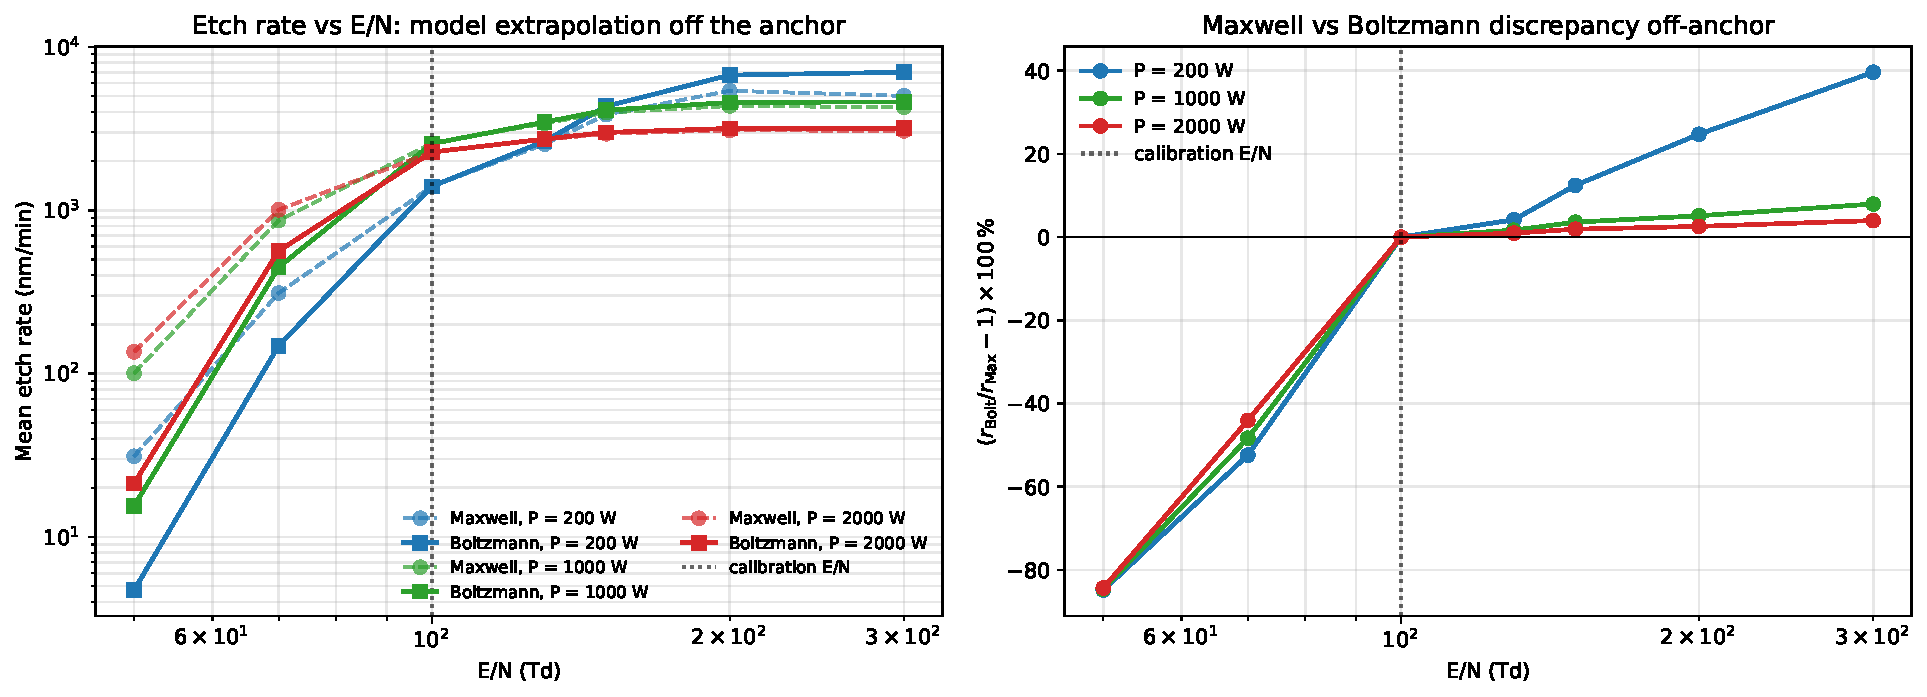
\includegraphics[width=0.9\linewidth]{figures/fig7_observability_sweep}
  \caption{Observable difference
  $\Delta_{\mathrm{obs}} = r_{\mathrm{Bolt}}/r_{\mathrm{Max}} - 1$
  between Maxwellian- and Boltzmann-calibrated models off the
  calibration axis. Left: $\Delta_{\mathrm{obs}}$ vs $E/N$ at
  $x_{\mathrm{Ar}} = 0$ and three absorbed powers. Right:
  $\Delta_{\mathrm{obs}}$ vs $x_{\mathrm{Ar}}$ at $E/N = 100\,$Td
  and two absorbed powers. The non-monotone $x_{\mathrm{Ar}}$
  response has its observability maximum at
  $x_{\mathrm{Ar}} \approx 0.30$, recommending this as the
  single-point discriminating experiment.}
  \label{fig:observability}
\end{figure}

The practical implication is that a single-condition calibration
against etch-rate measurements at the same
$(E/N, x_{\mathrm{Ar}})$ cannot identify the correct EEDF model
regardless of the number of absorbed-power values used. The
identifiability structure of
Section~\ref{sec:identifiability} permits any two EEDF hypotheses
lying on the same point of the manifold to produce identical
predictions at the calibration condition. Multi-condition
measurements are required to break the degeneracy, and the most
practical single-knob perturbation is Ar dilution. Compared with
pressure or flow sweeps, which perturb several model inputs
simultaneously (gas residence time, neutral density, gas-heating
profile), Ar dilution at fixed pressure and absorbed power changes
only the electron-kinetics input and changes it in the direction
that maximally resolves the attachment-tail depletion. A single
etch-rate measurement at $x_{\mathrm{Ar}} = 0.30$,
$p = 10\,$mTorr, $P \in [50,\,200]\,$W produces a predicted signal
$|\Delta_{\mathrm{obs}}|$ between $39\,\%$ and $47\,\%$, an order
of magnitude larger than typical etch-rate measurement noise. A
measurement of this type would lift the calibration degeneracy
identified in Section~\ref{sec:identifiability} and fix the
physical interpretation of the depletion parameter established in
Section~\ref{sec:boltzmann} with only one additional experimental
run beyond the existing two-anchor calibration.
